\documentclass[11pt,a4paper]{article}
\usepackage[margin=0.85in,top=1in,bottom=1in]{geometry}
\usepackage{amsmath,amssymb,amsfonts}
\usepackage{graphicx}
\usepackage{float}
\usepackage{enumitem}
\usepackage{microtype}
\usepackage{caption}
\usepackage[hidelinks]{hyperref}
\usepackage[most,breakable]{tcolorbox}
\tcbuselibrary{breakable,skins}
\usepackage[utf8]{inputenc}
\usepackage[T1]{fontenc}
\usepackage{lmodern}
\captionsetup{font=small,labelfont=bf,skip=4pt}
\setlist{leftmargin=1.5em,topsep=2pt}

%% Breakable card — prevents content cutoff across pages
\newtcolorbox{solcard}[3]{
  breakable, enhanced,
  colback=white, colframe=gray!50, arc=2pt,
  title={\textbf{#1}\hfill\textsf{\small #3\,pts}},
  fonttitle=\normalsize\sffamily\bfseries,
  before upper={\small\textit{#2}\par\smallskip\hrule height 0.4pt\smallskip},
  top=4pt, bottom=6pt, left=7pt, right=7pt,
  parbox=false,
}

\title{\textbf{Photography problems --- Solution}}
\author{\normalsize X26 (2026) — English translation}
\date{}
\begin{document}\maketitle\vspace{-0.5em}
\begin{solcard}{A1}{Find the position and shape of the wire if its length is minimal.}{2.00}

The image of the wire is symmetrical about $Y$, so the wire lies in the $xy$ plane. Note that each point of the wire gives a point on the screen (if the camera is focused on this point) or a circle (from the likeness of cones).


Let's find the position of the circle and its dimensions for the point with coordinates $(x,y,0)$. Coordinates of the center of the circle from the similarity of triangles: $$\left(Y,Z\right) = \left(\cfrac{yl}{x},0\right).$$For diameter: $$\cfrac{d}{D} = \cfrac{a-l}{a} = 1-\cfrac{l}{a}.$$Substitute value $1/a$ from the thin lens formula. $$\cfrac{d}{D} = 1-l\left(\cfrac{1}{f}-\cfrac{1}{x}\right) = 1 - \cfrac{l\left(x-f\right)}{fx}.$$Find dependence $d$ from $Y$ for $Y>0$.


By condition $\tan \theta = k$. $$d = 2Y\sin\theta = \frac{2k}{\sqrt{1+k^2}} \cdot Y = \gamma Y = \gamma \cdot \cfrac{yl}{x},$$where $\gamma = \frac{2k}{\sqrt{1+k^2}}$. Substituting this into the previously obtained expression for $d$. $$\cfrac{d}{D} = \cfrac{\gamma yl}{Dx} = 1 - \cfrac{l\left(x-f\right)}{fx}$$Express $y(x)$: $$y = \cfrac{Dx}{\gamma l} - \cfrac{D\left(x-f\right)}{\gamma f} = \cfrac{D}{\gamma} - \cfrac{Dx}{\gamma} \left(\cfrac{1}{f}-\cfrac{1}{l}\right) = \cfrac{D}{\gamma} - \cfrac{Dx\left(l-f\right)}{\gamma fl}.$$Note, that since wire place in region $x>0$ and image point wire in center screen be point, that camera focus on one from point wire, therefore $l > f$. Note, that we consider case $a\geqslant l$, if this not thus, that the same equation remains valid, but the sign of $d$ flips. That is, for the consideration $a < l$ sufficiently in obtain expression change sign $\gamma$. Thus we obtain, that possible position point determine form image: $$y = \pm\cfrac{D\left(l-f\right)\sqrt{1+k^2}}{2k lf} \left(\cfrac{lf}{l-f}-x\right).$$Perhaps the wire contains more sections, the images of which overlap with the images of points on these lines, but then the wire will have a greater length, which contradicts the condition. Therefore, it lies completely on these straight lines.


Note that the angular size of the parts of straight lines $1'$ and $2'$ is less than $90^\circ$, therefore they can give in the image a circle with a limited segment of the positions of the centers; even for a fixed angular size, the length of the wire in sections $1$ and $2$ will always be less, therefore the wire has the shape of an angle from the segments $1$ and $2$:

\par\smallskip\noindent\textbf{Answer:} $$y = \pm\cfrac{D\left(l-f\right)\sqrt{1+k^2}}{2k lf} \left(\cfrac{lf}{l-f}-x\right)$$for $x \in \left[0, \cfrac{lf}{l-f}\right]$.
\begin{figure}[H]
  \centering
  
\includegraphics[width=0.72\textwidth]{T3_S_EN_assets/fig1.jpg}
\end{figure}
\begin{figure}[H]
  \centering
  
\includegraphics[width=0.72\textwidth]{T3_S_EN_assets/fig2.jpg}
\end{figure}
\begin{figure}[H]
  \centering
  
\includegraphics[width=0.72\textwidth]{T3_S_EN_assets/fig3.jpg}
\end{figure}
\end{solcard}

\begin{solcard}{B1}{Using a compass and straight edge, draw a straight line parallel to the direction of the puck's speed.}{2.00}

Let's understand how an image is formed. Let's enter the coordinates $XY$, which are attached to the puck and indicate the position of the point on it, and $xy$, which determine the position in the photograph. Let the speed of the line that the camera films at a particular moment is equal to to $u$; the center of the puck was photographed at point $(x_0,y_0)$ and at time $t_0$.


The angle between the speed of the puck and the $x$ axis will be denoted by $\alpha$. Let's find the coordinates in the photograph for an arbitrary point on the puck $(X,Y)$. The moment of photographing this point: $$t = t_0 + \frac{Y}{u-v\sin\alpha}.$$Coordinate equal: $$x = x_0 + X + v\cos\alpha\left(t-t_0\right) = x_0+X+\frac{v\cos\alpha}{u-v\sin\alpha}Y,$$$$y = y_0 + u\left(t-t_0\right) = y_0+\frac{u}{u-v\sin\alpha}Y.$$Note, that transformation coordinate linearly. Means, straight on puck be straight on image. Construct possible direction velocity. Obtain image straight $X=0$, for this conduct horizontal straight, image $X = 0$ be straight pass through through center intersection horizontal straight with image puck (since for record $Y$ and correspondingly $y$ coordinate $x$ and $X$ differ only by a constant).


Now we get a segment of length equal to the diameter. To do this, it is enough to draw a horizontal segment through the center of the image $X=0$.


Then there are two options for how photography can take place depending on the speed of the puck. If $u > v\sin\alpha$, then the top point of the image is the top point of the washer. And accordingly, vice versa, if $u < v\sin\alpha$, then the top point of the image is the bottom point of the washer. Let's draw the initial and final states of the puck depending on the speed ratio. $u > v\sin\alpha:$


$u < v\sin\alpha:$


Note that in this way we can obtain the possible direction of the speed: we obtain the point $A$ by constructing a vertical segment of length $d$ with one end at the top point of the image of the puck, the speed will be directed along $\overrightarrow{AA'}$.

\begin{figure}[H]
  \centering
  
\includegraphics[width=0.72\textwidth]{T3_S_EN_assets/fig4.jpg}
\end{figure}
\begin{figure}[H]
  \centering
  
\includegraphics[width=0.72\textwidth]{T3_S_EN_assets/fig5.jpg}
\end{figure}
\begin{figure}[H]
  \centering
  
\includegraphics[width=0.72\textwidth]{T3_S_EN_assets/fig6.jpg}
\end{figure}
\begin{figure}[H]
  \centering
  
\includegraphics[width=0.72\textwidth]{T3_S_EN_assets/fig7.jpg}
\end{figure}
\begin{figure}[H]
  \centering
  
\includegraphics[width=0.72\textwidth]{T3_S_EN_assets/fig8.jpg}
\end{figure}
\begin{figure}[H]
  \centering
  
\includegraphics[width=0.72\textwidth]{T3_S_EN_assets/fig9.jpg}
\end{figure}
\end{solcard}

\begin{solcard}{B2}{Using an additional ruler with divisions, find the speed modulus of the puck.}{1.00}

It remains to determine the velocity module. We plotted the displacement of point $A$ during the time of shooting the puck $\tau$. We can express this time in terms of the total photographing time $T$.


$$\tau = \frac{l}{L}T=0.5\cdot T = 5\text{ ms}$$By photograph can determine displacement puck: $$\frac{S_1}{d} = 2.24;\qquad\frac{S_2}{d} = 1.00.$$$$S_1 = 17.1\text{ cm};\qquad S_2 = 7.62\text{ cm}$$Remain calculate quantity velocity $v = S/\tau$.

\par\smallskip\noindent\textbf{Answer:} $$v_1 = 34.1\text{ m/s};\qquad v_2 = 15.2\text{ m/s}$$
\begin{figure}[H]
  \centering
  
\includegraphics[width=0.72\textwidth]{T3_S_EN_assets/fig10.jpg}
\end{figure}
\end{solcard}

\begin{solcard}{C1}{Show that the linear magnification of a pinhole camera is constant and find $\alpha$.}{0.50}

Let's consider how an image of a single point is formed.


From the similarity we obtain: $$\frac{R}{r} = \frac{l}{L}.$$The resulting expression does not depend on the position of the point, so distortion is not observed.

\par\smallskip\noindent\textbf{Answer:} $$\alpha = \frac{l}{L}$$
\begin{figure}[H]
  \centering
  
\includegraphics[width=0.72\textwidth]{T3_S_EN_assets/fig11.jpg}
\end{figure}
\end{solcard}

\begin{solcard}{C2}{Draw a high-quality view of the photograph of part of the notebook sheet shown in the figure below, in cases $\beta > 0$ (positive distortion) and $\beta < 0$ (negative distortion). Consider that $\alpha > 0$.}{0.50}

In the case of $\beta > 0$ the image of the graph paper (we present it for a more detailed illustration) and the square will look like:


In case of $\beta < 0$:

\begin{figure}[H]
  \centering
  
\includegraphics[width=0.72\textwidth]{T3_S_EN_assets/fig12.jpg}
\end{figure}
\begin{figure}[H]
  \centering
  
\includegraphics[width=0.72\textwidth]{T3_S_EN_assets/fig13.jpg}
\end{figure}
\begin{figure}[H]
  \centering
  
\includegraphics[width=0.72\textwidth]{T3_S_EN_assets/fig14.jpg}
\end{figure}
\begin{figure}[H]
  \centering
  
\includegraphics[width=0.72\textwidth]{T3_S_EN_assets/fig15.jpg}
\end{figure}
\begin{figure}[H]
  \centering
  
\includegraphics[width=0.72\textwidth]{T3_S_EN_assets/fig16.jpg}
\end{figure}
\end{solcard}

\begin{solcard}{C3}{Determine the coefficients $\alpha$ and $\beta$ in this case. What kind of distortion is observed in such a system: positive ($\alpha$ and $\beta$ of the same sign) or negative ($\alpha$ and $\beta$ of different signs)?}{2.00}

Note that we are considering third-order effects for paraxial rays, so all formulas can be expanded to third order. Let's find the connection between $R$ and $r$.


Let's express the dimensions through the angles: $$R = l\tan\varphi;$$$$r = \left(L - h\right)\tan\varphi + h\tan\psi.$$Relation angle: $$n\sin\psi = \sin\varphi.$$$$\psi = \arcsin\left(\frac{\sin\varphi}{n}\right) \approx \arcsin\left(\frac{\varphi}{n}-\frac{\varphi^3}{6n}\right)\approx\frac{\varphi}{n}-\frac{\varphi^3}{6n} + \frac{\varphi^3}{6n^3} = \frac{\varphi}{n}-\frac{\varphi^3\left(n^2-1\right)}{6n^3}$$$$\tan\psi \approx \psi + \frac{\psi^3}{3}\approx\frac{\varphi}{n}-\frac{\varphi^3\left(n^2-1\right)}{6n^3} + \frac{\varphi^3}{3n^3} = \frac{\varphi}{n}-\frac{\varphi^3\left(n^2-3\right)}{6n^3}$$$$\varphi = \arctan\left(\frac{R}{l}\right)\approx\frac{R}{l}-\frac{R^3}{3l^3}$$$$\tan\psi \approx \frac{R}{nl} - \frac{R^3}{3l^3n}-\frac{R^3\left(n^2-3\right)}{6l^3n^3} = \frac{R}{nl} - \frac{R^3\left(n^2-1\right)}{2l^3n^3}$$$$r = \frac{L-h}{l}R+\frac{h}{nl}R - \frac{h\left(n^2-1\right)}{2l^3n^3}R^3=\frac{nL-\left(n-1\right)h}{nl}R - \frac{h\left(n^2-1\right)}{2l^3n^3}R^3.$$ Introduce notation: $$A = \frac{nL-\left(n-1\right)h}{nl};\qquad B = \frac{h\left(n^2-1\right)}{2l^3n^3}.$$$$r=AR-BR^3$$$$r \approx A\left(\alpha r + \beta r^3\right) - B\alpha^3r^3 = A\alpha r + \left(A\beta - B\alpha^3\right)r^3$$Equate the coefficients at like powers and express sought coefficients: $$\begin{cases} A\alpha = 1;\\ A\beta - B\alpha^3 = 0. \end{cases}$$$$\alpha = \frac{1}{A} = \frac{nl}{nL-\left(n-1\right)h}$$$$\beta = \frac{B}{A^4} = \frac{hnl\left(n^2-1\right)}{2\left(nL-\left(n-1\right)h\right)^4}$$

\par\smallskip\noindent\textbf{Answer:} Positive distortion is observed. $$\alpha = \frac{nl}{nL-\left(n-1\right)h}\qquad\qquad\beta = \frac{hnl\left(n^2-1\right)}{2\left(nL-\left(n-1\right)h\right)^4}$$
\begin{figure}[H]
  \centering
  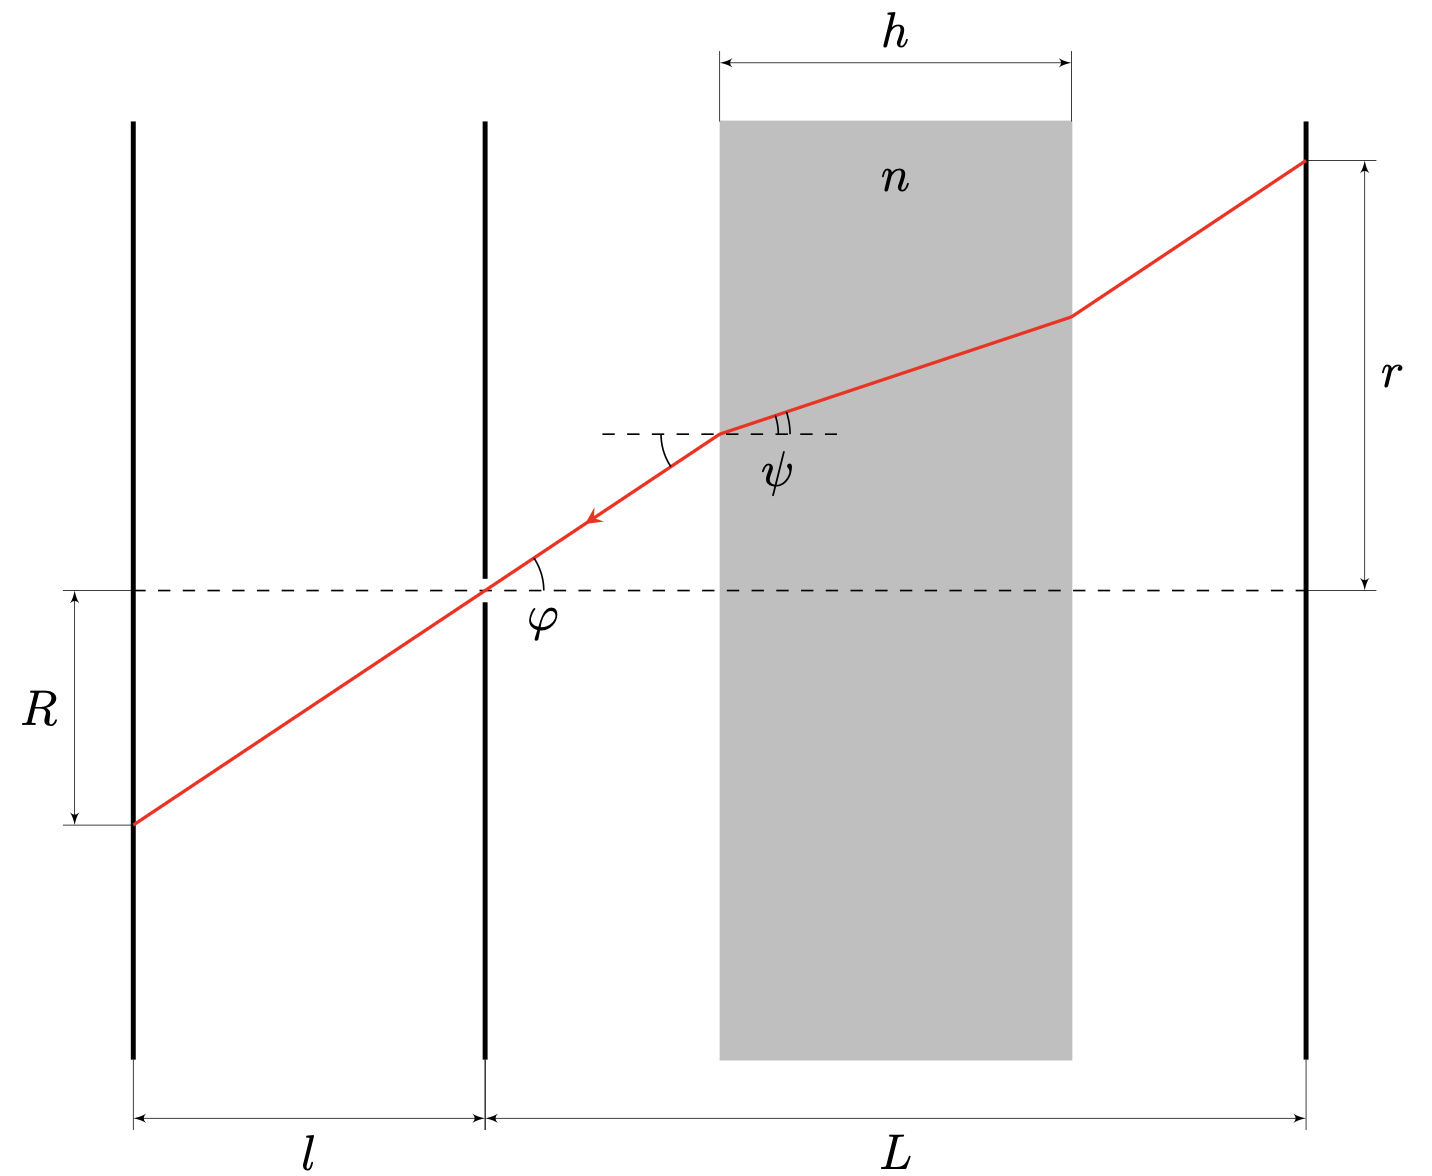
\includegraphics[width=0.72\textwidth]{T3_S_EN_assets/fig17.jpg}
\end{figure}
\end{solcard}

\end{document}